\section{The K-mer Representation Quality} \label{sec:K_mer_Representation}

Investigation on the anomalies resulted in two persistent clustering errors \autoref{fig:PCA_Cluster_Knee_4} \textbf{\textsf{B}} and \textbf{\textsf{D}}. To evaluate if the method is suitable for the clustering of \gls{IAV} possible error sources are discussed.

% \begin{figure}[!hbt]
%     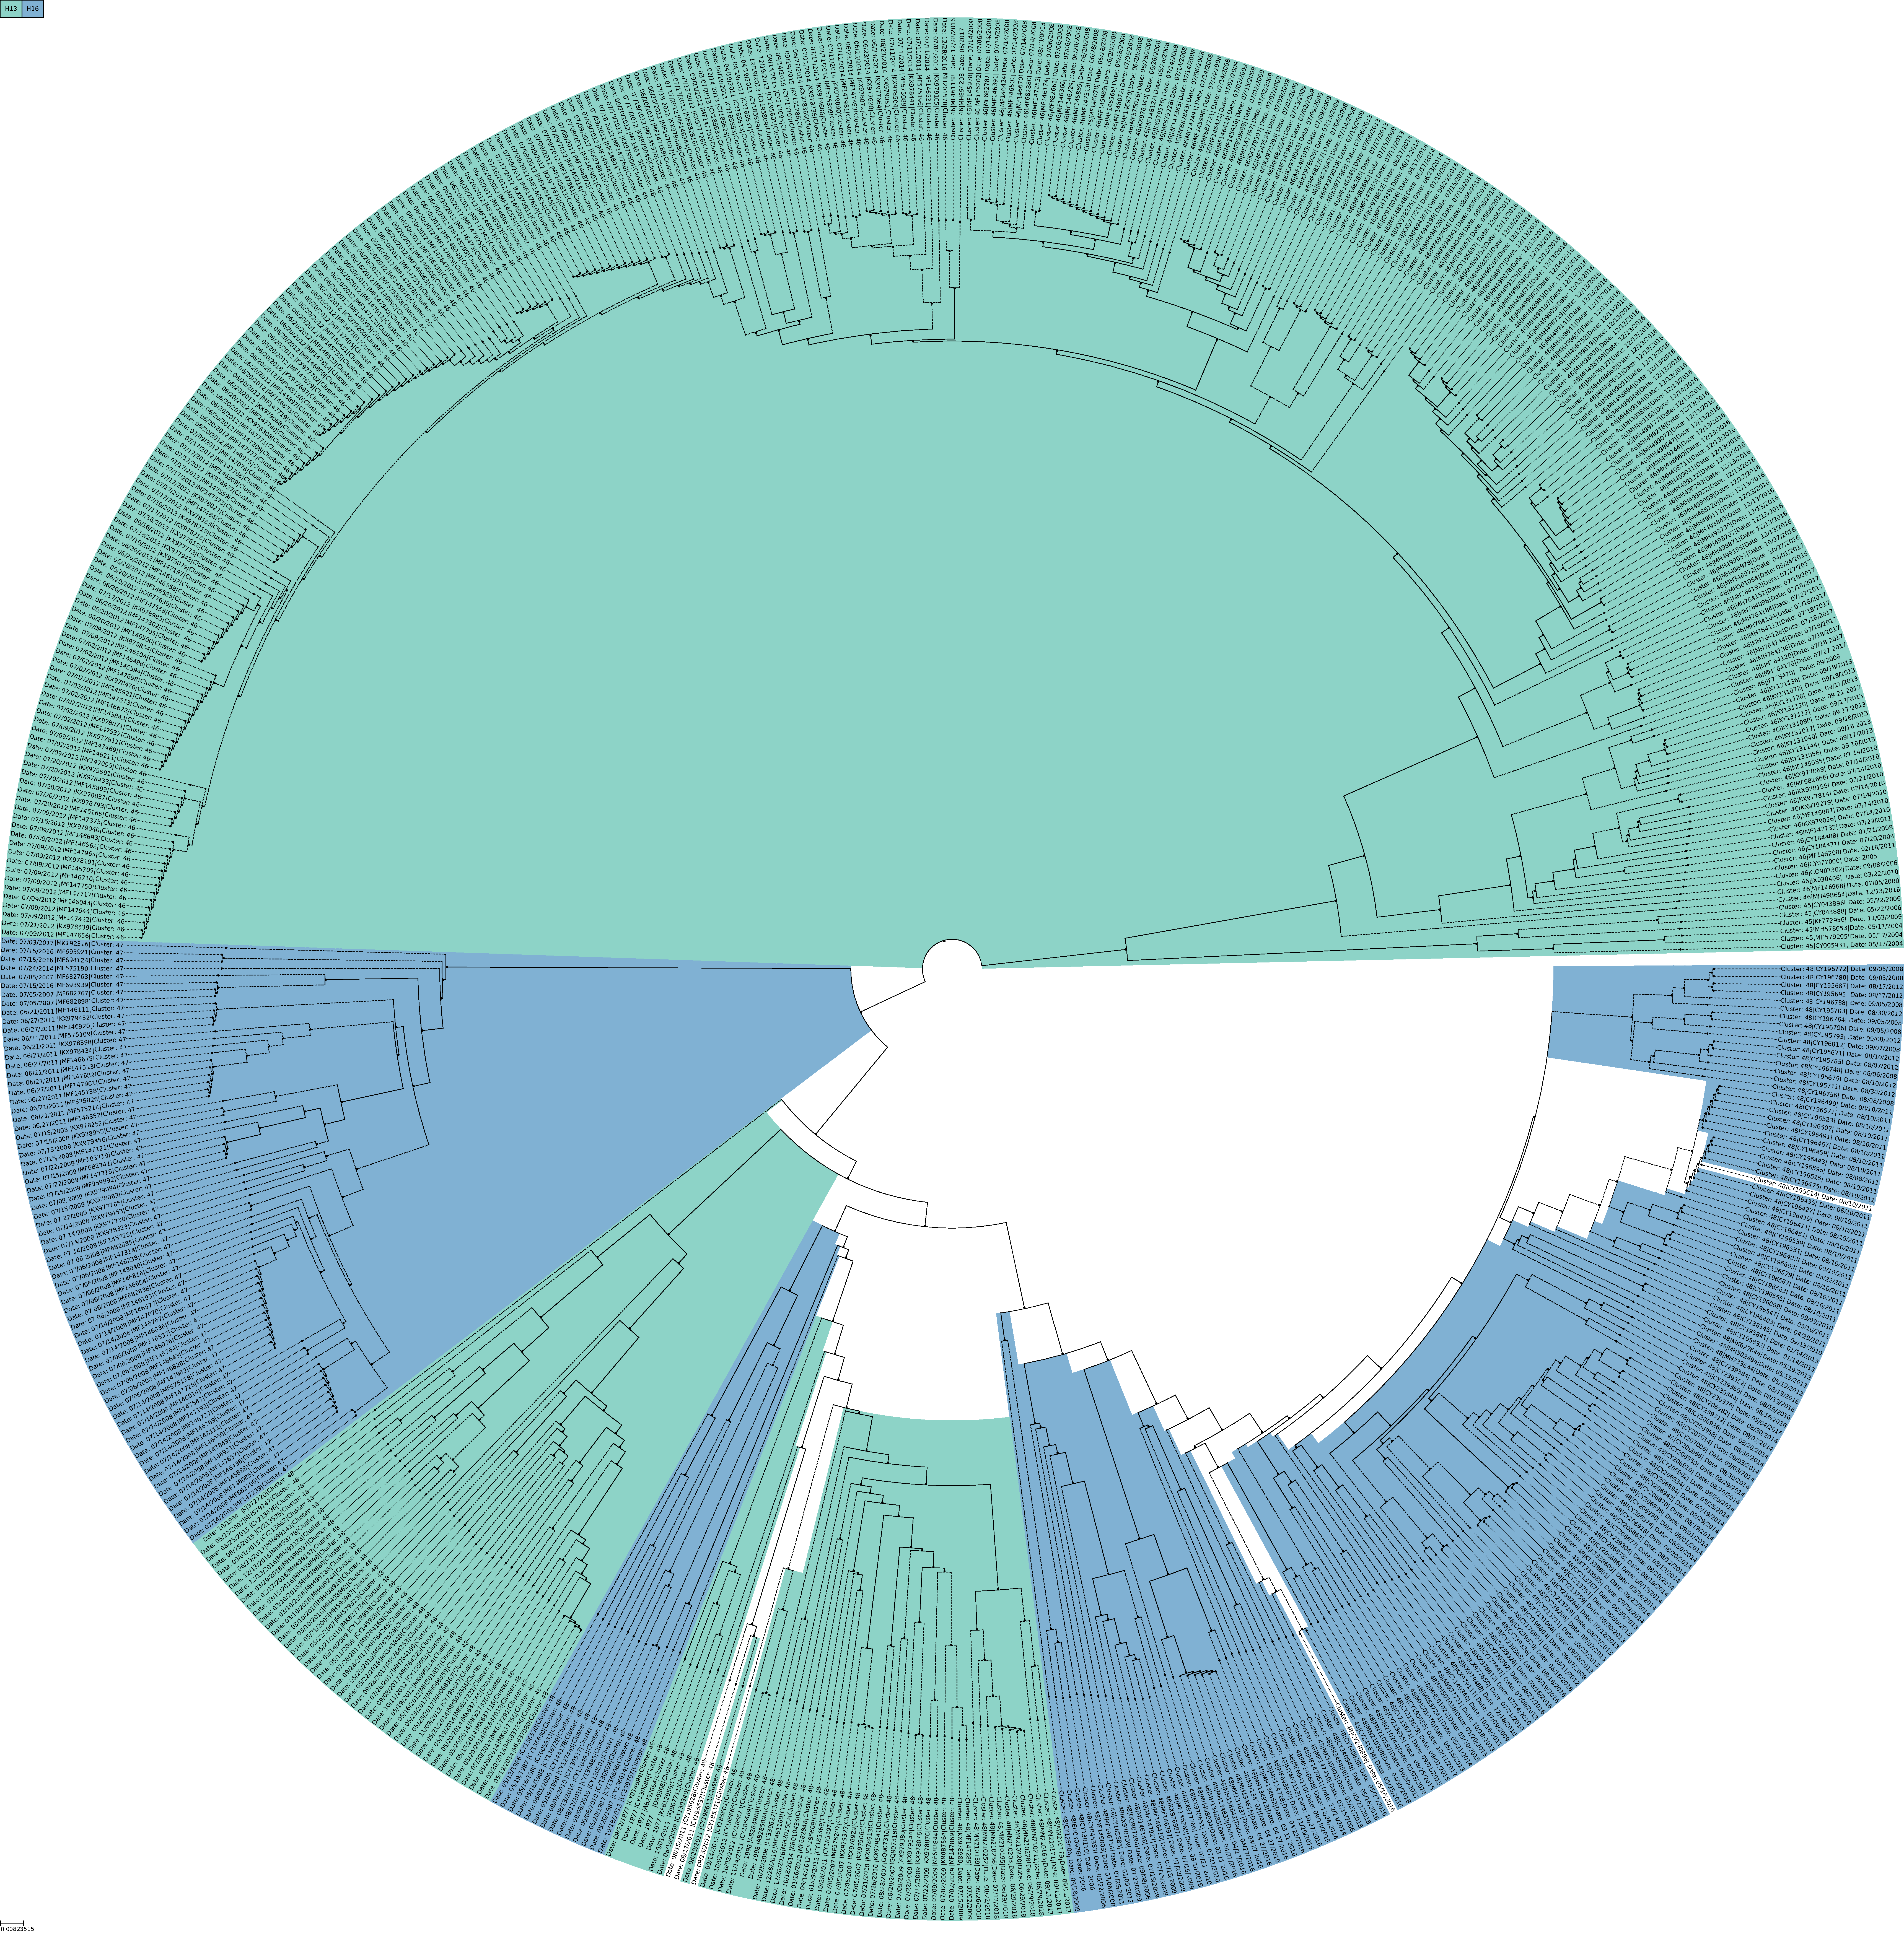
\includegraphics[width=\dimexpr\textwidth-2\fboxsep-2\fboxrule,fbox]{PCA/Clustertree_Segment_4_H_Knee_Zoom.pdf}
%     \caption[H13/H16 Simple Clustering Example with \Acrshort{PCA}]{\textbf{H13/H16 Simple Clustering Example with \Acrshort{PCA}.} .}
%     \label{fig:PCA_Clusteree_Knee_Zoom}
% \end{figure}

% \begin{figure}[!hbt]
%     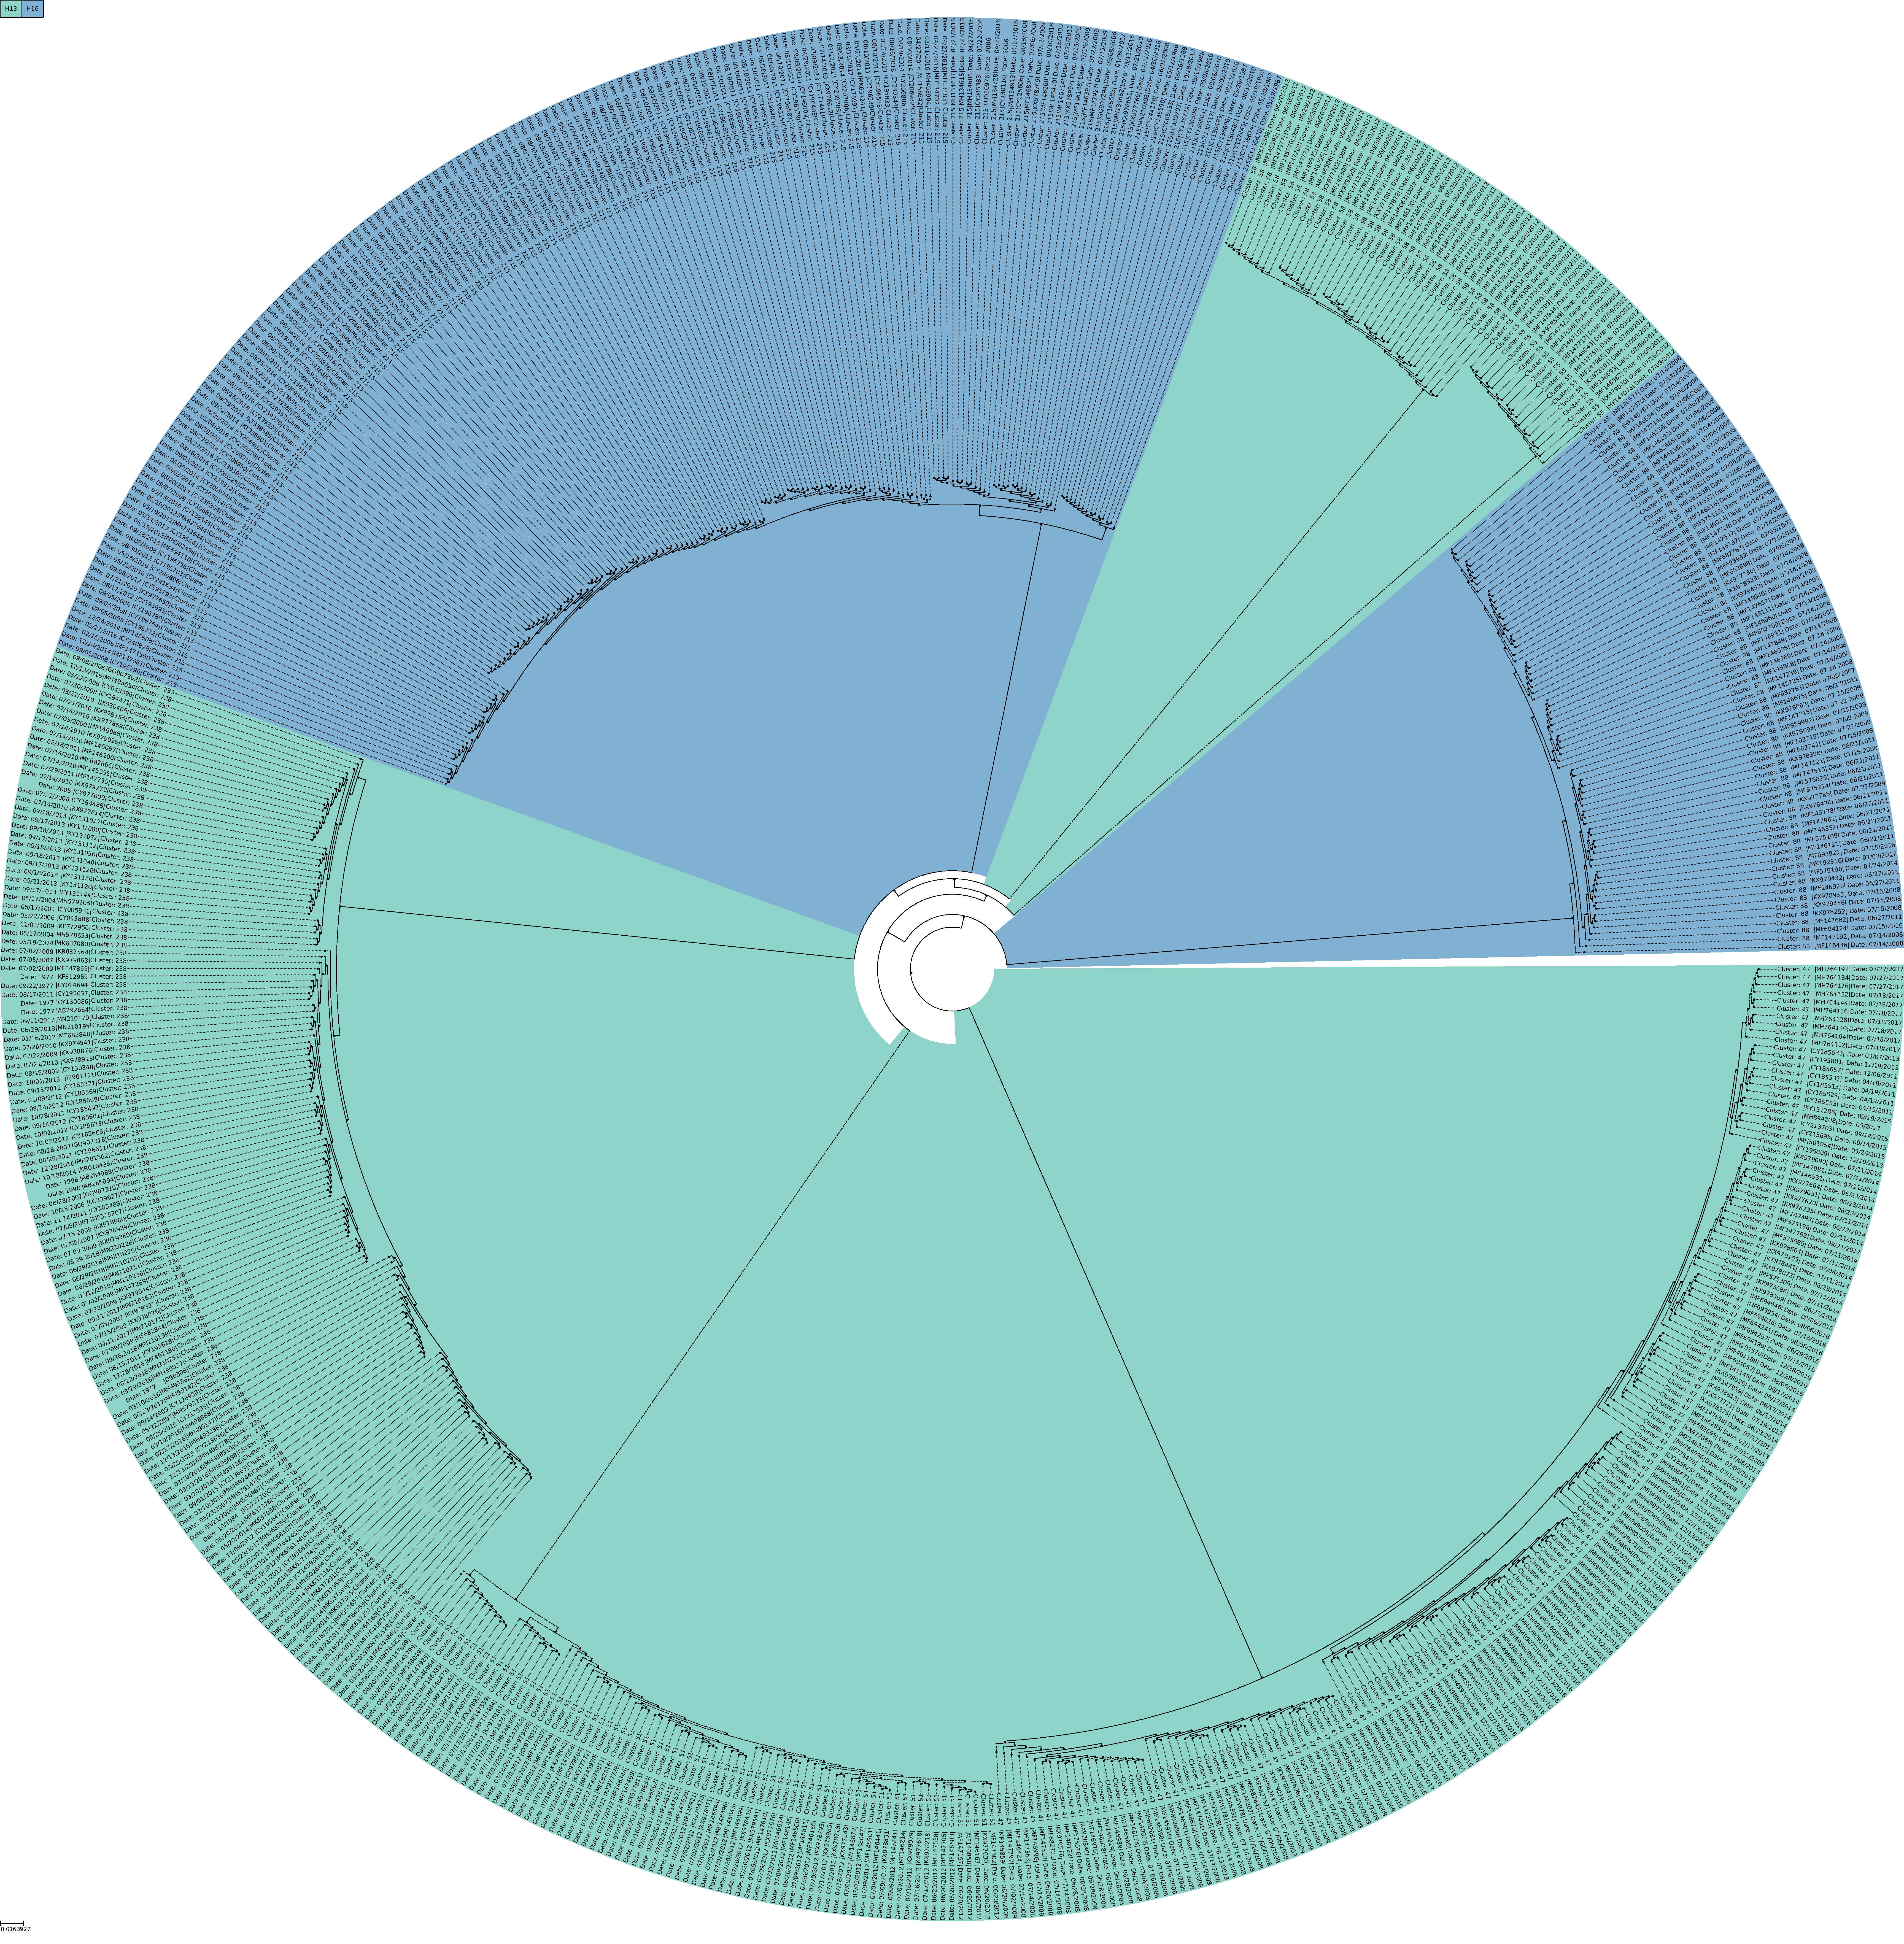
\includegraphics[width=\dimexpr\textwidth-2\fboxsep-2\fboxrule,fbox]{UMAP/Clustertree_Segment_4_H_Knee_Zoom.pdf}
%     \caption[H13/H16 Simple Clustering Example with \Acrshort{UMAP}]{\textbf{H13/H16 Simple Clustering Example with \Acrshort{UMAP}.} .}
%     \label{fig:UMAP_Clusteree_Knee_Zoom}
% \end{figure}

% \begin{figure}[!hbt]
%     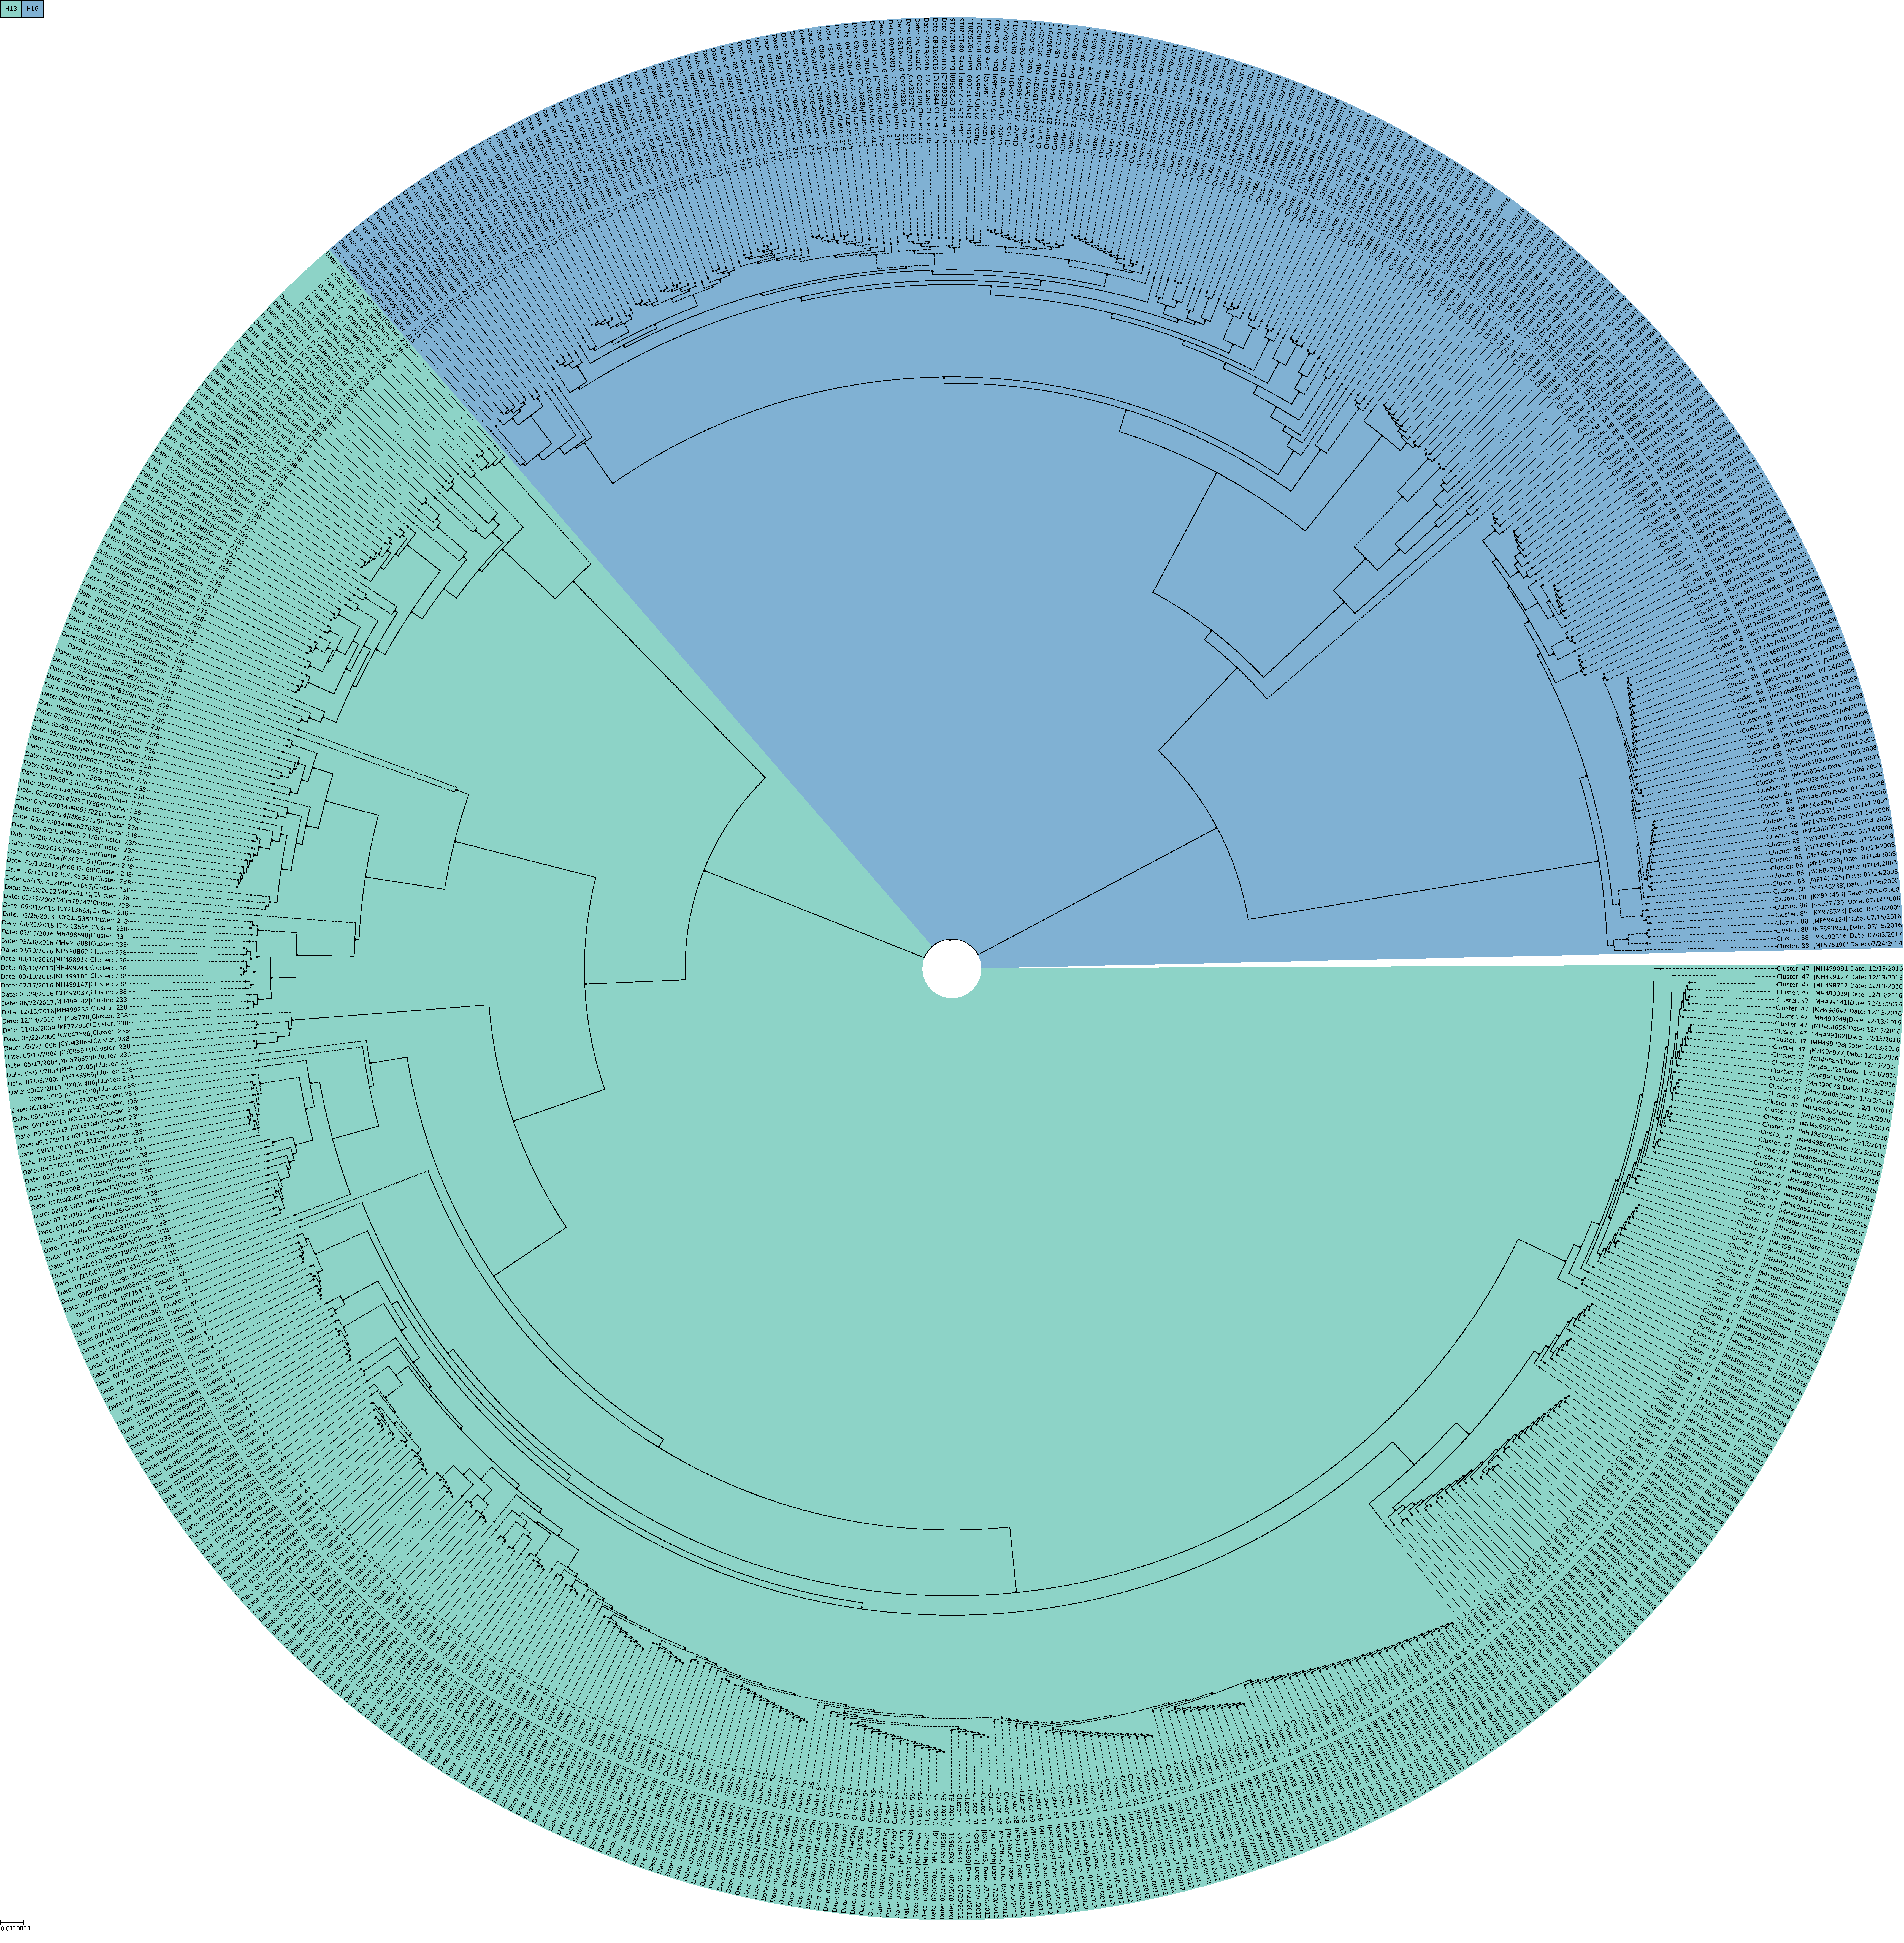
\includegraphics[width=\dimexpr\textwidth-2\fboxsep-2\fboxrule,fbox]{UMAP/Guidetree_Segment_4_H_Focus.pdf}
%     \caption[H13/H16 Simple Clustering Example with \Acrshort{MSA}]{\textbf{H13/H16 Simple Clustering Example with \Acrshort{MSA}.} .}
%     \label{fig:Guidetree_Focus}
% \end{figure}

\begin{figure}[!hbt]
    \centering
    \begin{tikzpicture}
        \node[anchor=south west,inner sep=0] (image) at (0,0) {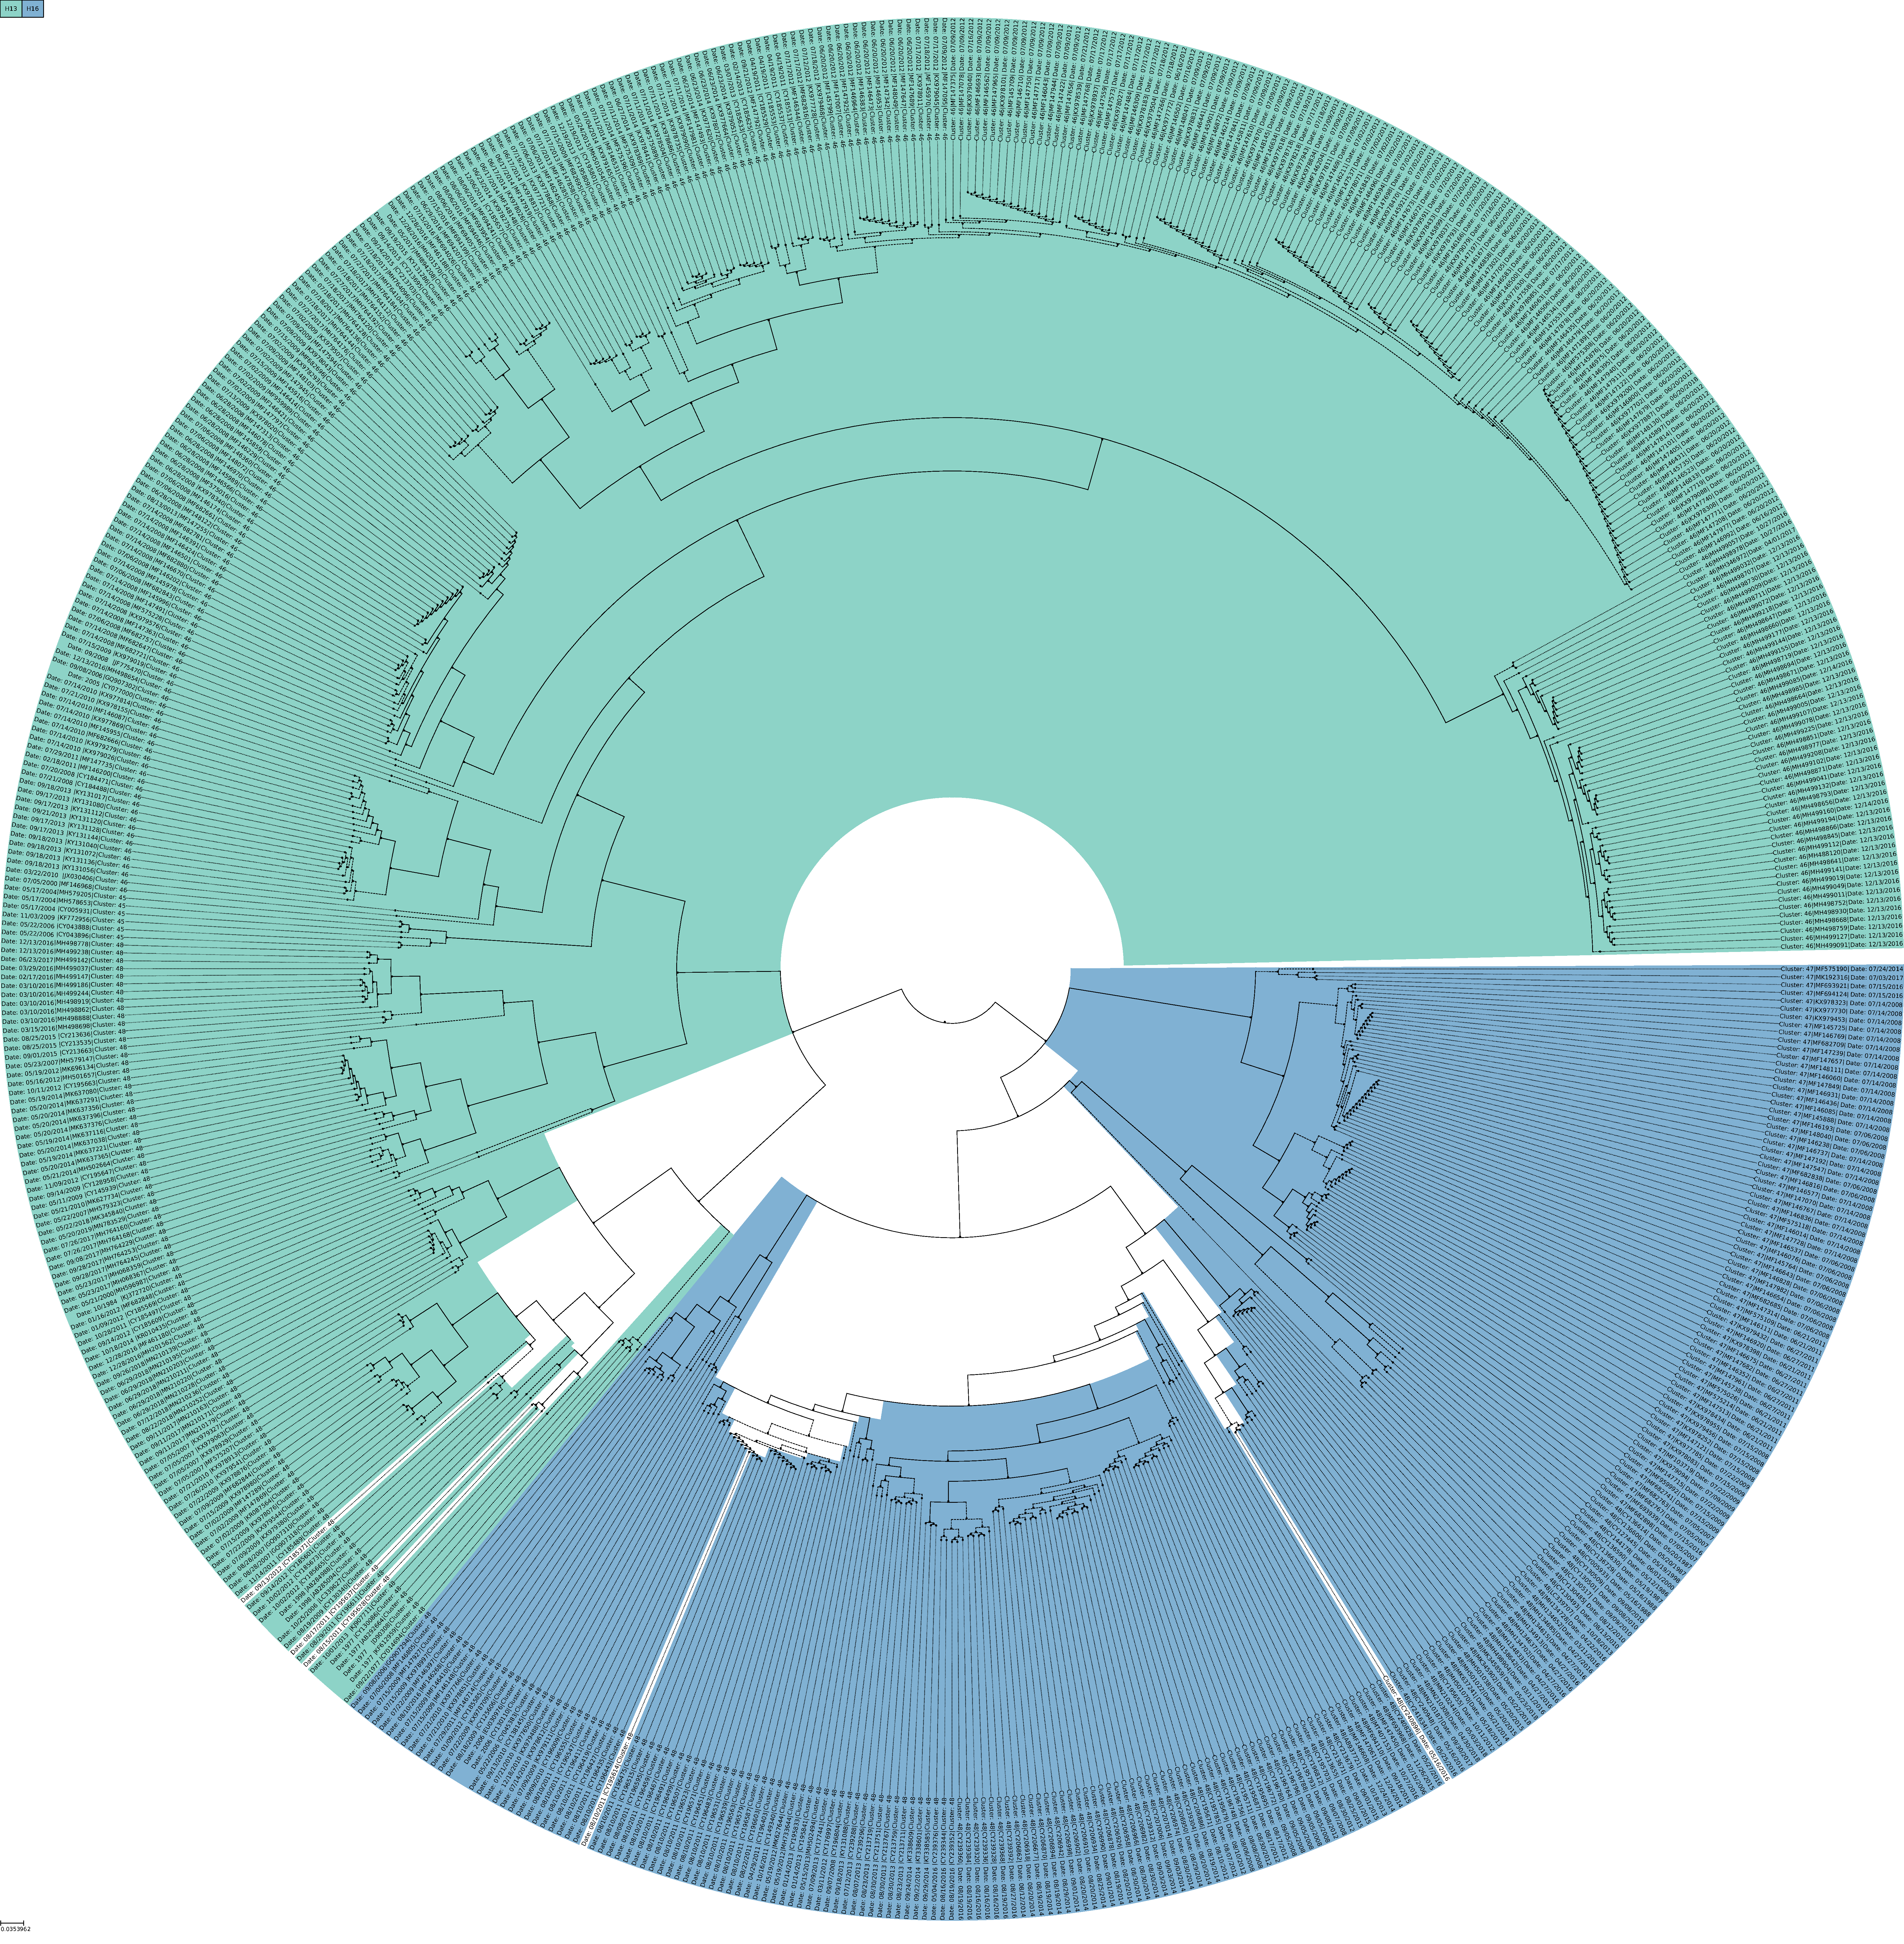
\includegraphics[width=\textwidth]{PCA/Precalculated_Segment_4_H_Cosine.pdf}};
        \begin{scope}[x={(image.south east)},y={(image.north west)}]
            \draw[step=10mm,help lines] (0,0) grid (1,1);
        \end{scope}
    \end{tikzpicture}
    \caption[H13/H16 Precalculated \Acrshort{UPGMA} Tree (cosine)]{\textbf{H13/H16 Precalculated \Acrshort{UPGMA} Tree (cosine).} .}
    \label{fig:Precalculated_Cosine}
\end{figure}

By building a \gls{UPGMA} tree on the non reduced segment 4 k-mer frequency vectors of the H13 and H16 subtypes the unbiased relation of sequences from these subtypes can be analyzed (\autoref{sec:MAFFT}). Also the fundamental use of k-mer frequencies can be validated or rejected. 
\begin{figure}[!hbt]
    \centering
    %\begin{adjustbox}{minipage=\dimexpr\textwidth-2\fboxsep-2\fboxrule,fbox}
    \begin{subfigure}[t]{0.38\textwidth}
        \caption{}
        %\label{subfig:} 
        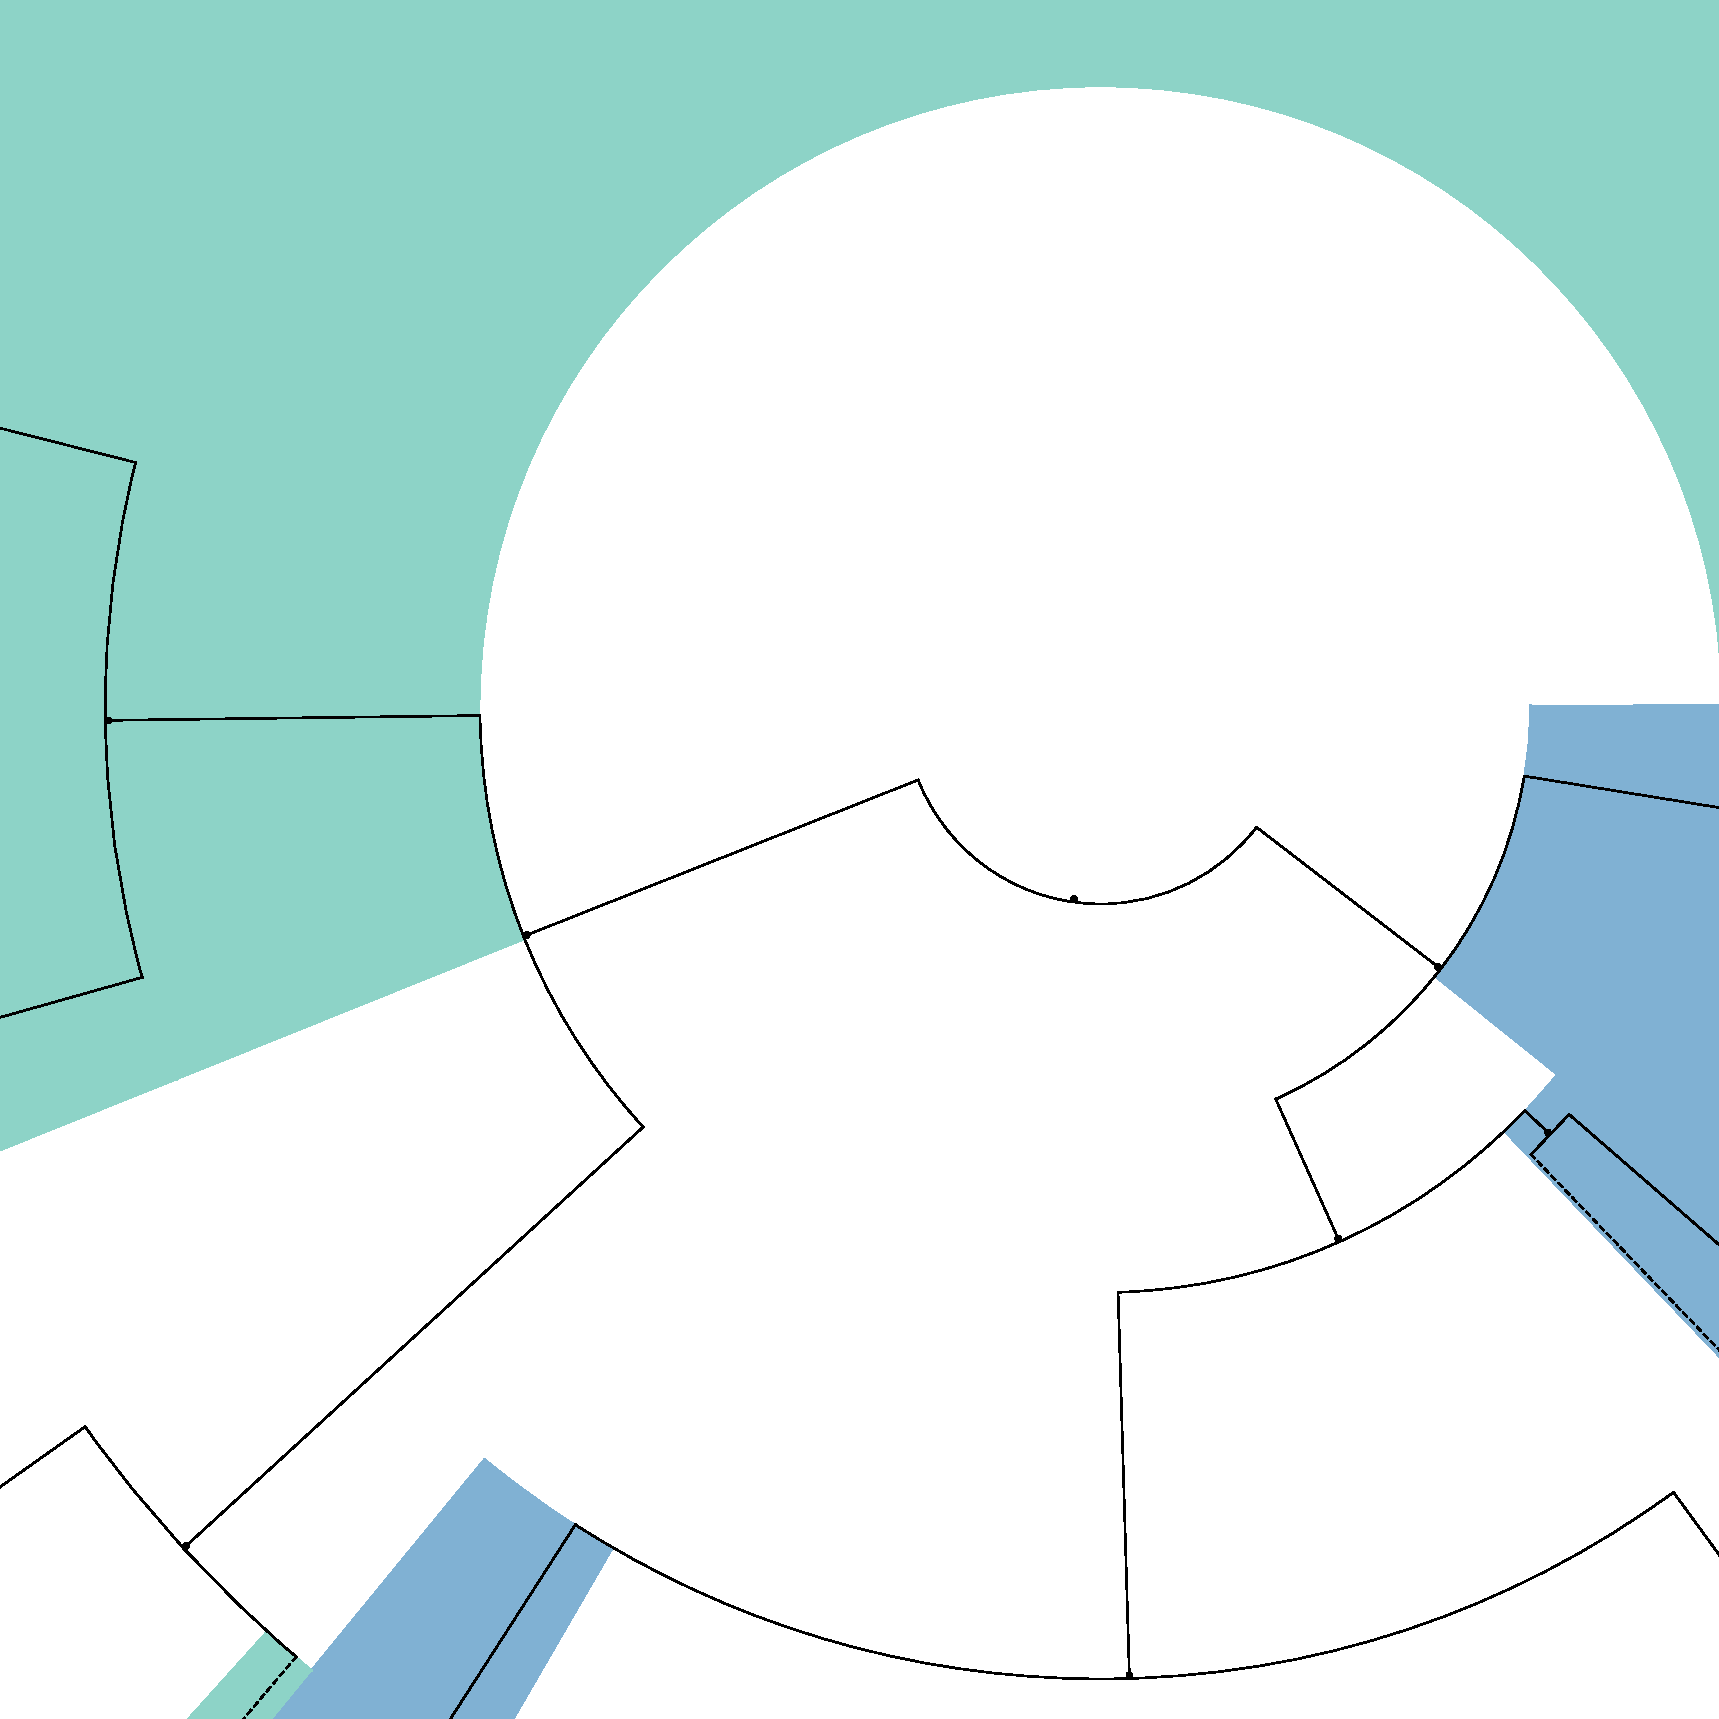
\includegraphics[width=\textwidth]{Graphics/root.pdf}
    \end{subfigure}
    \hfill
    \begin{subfigure}[t]{0.38\textwidth}
        \caption{}
        %\label{subfig:}
        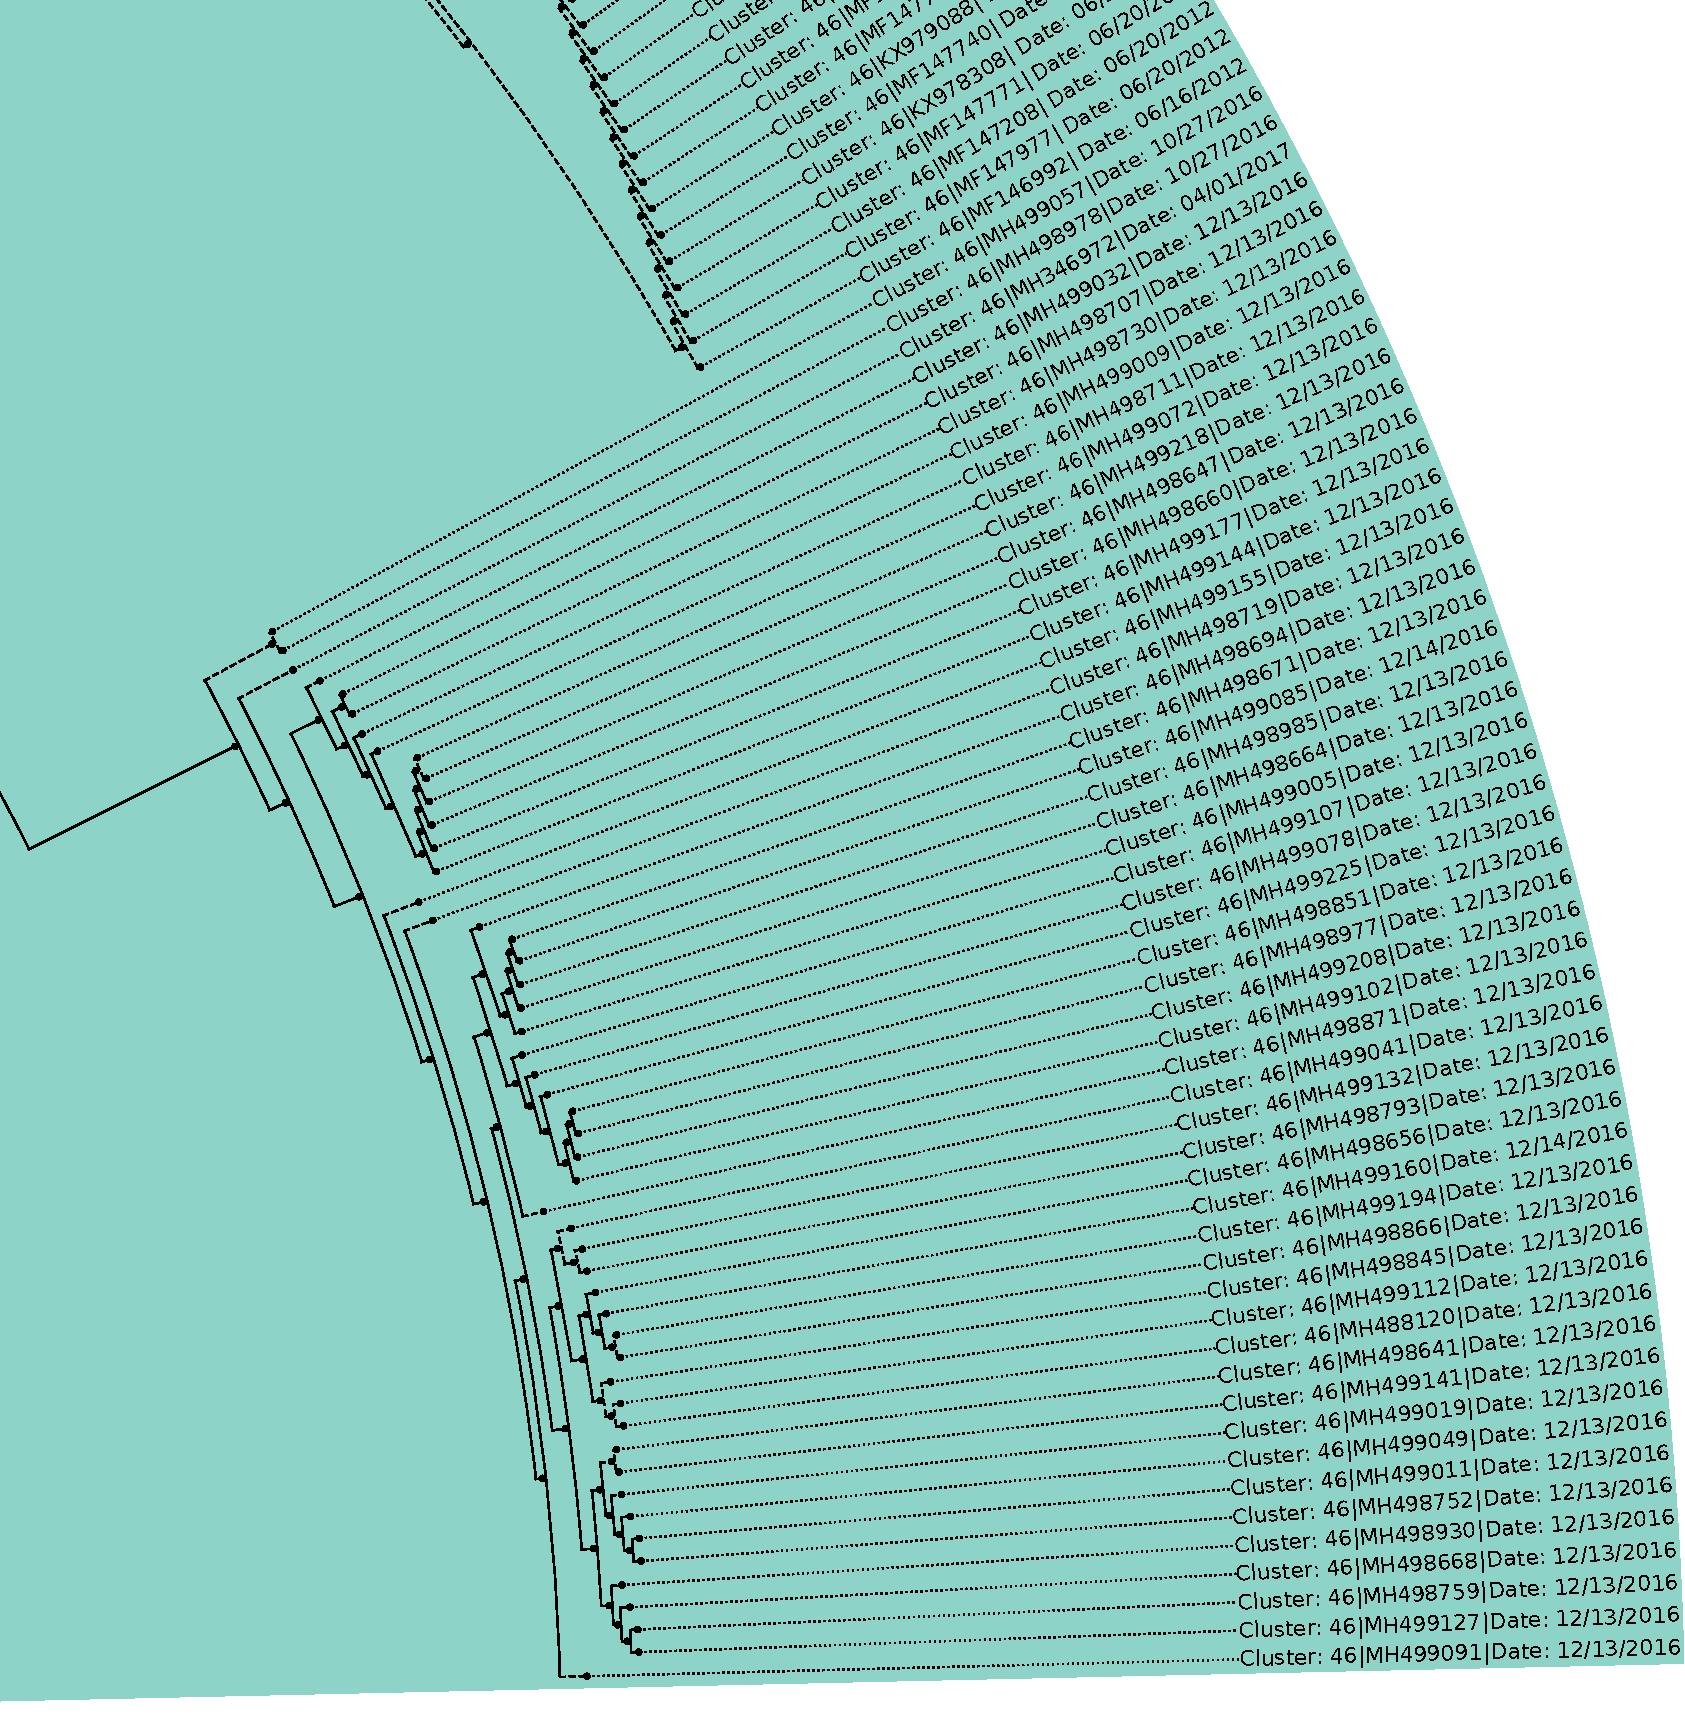
\includegraphics[width=\textwidth]{Graphics/identical.pdf}
    \end{subfigure}
    \hfill
    \begin{subfigure}[t]{0.19\textwidth}
        \caption{}
        %\label{subfig}
        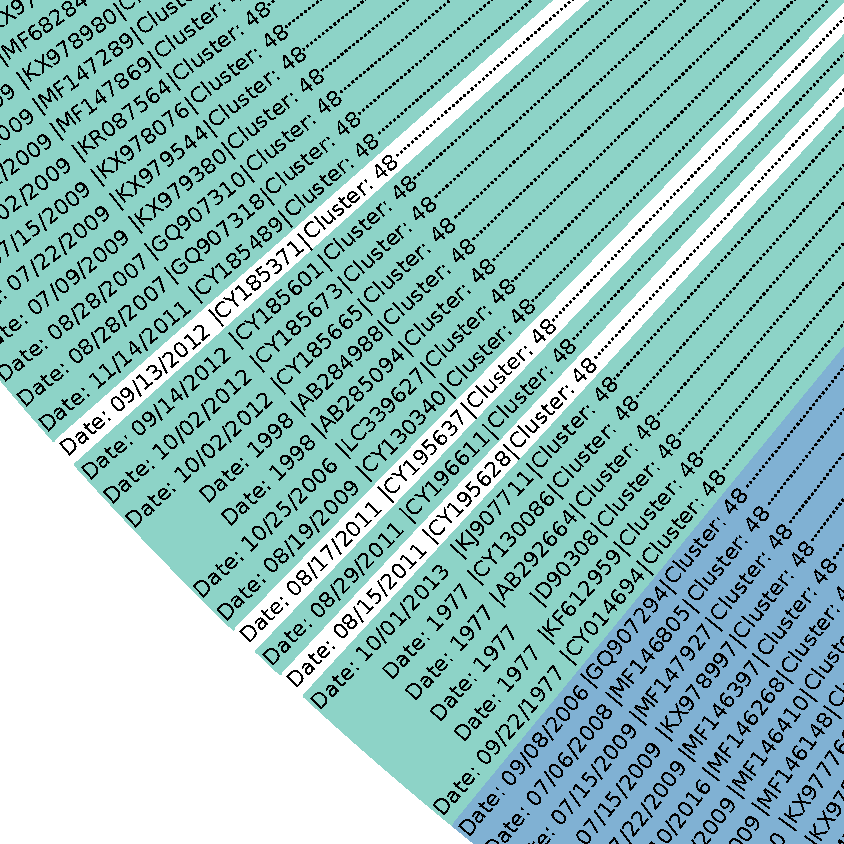
\includegraphics[width=\textwidth]{Graphics/unclassi_blue.pdf}
        \\[2mm]
        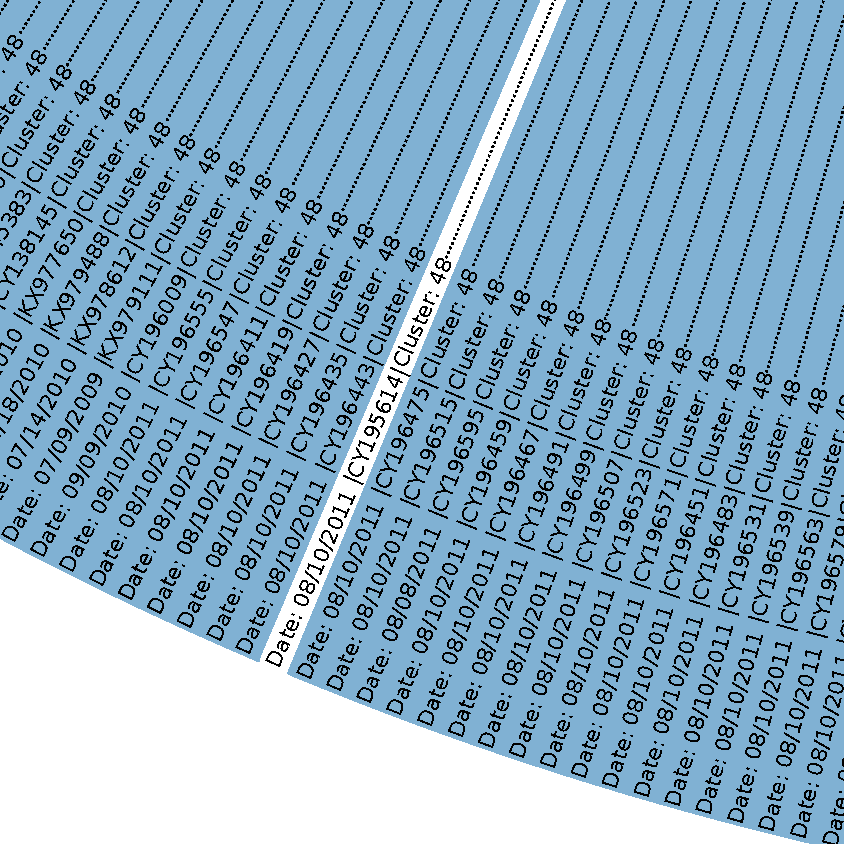
\includegraphics[width=\textwidth]{Graphics/unclassi_green.pdf}
    \end{subfigure}   
    \caption[]{}
    \label{fig:}
\end{figure}

%frage is hier welche Methode die bessere representation ausstrahlt, sprich UMAP vgl. precalc ja/nein? dann PCA vgl precalc passt? ja/nein?